% Pre-defense presentation — DNA language modeling with adaptive recursive tokenization.
% Build:  `make predefense`  (xelatex + polyglossia, matches thesis toolchain).
\documentclass[aspectratio=169,xcolor=table]{beamer}

\usepackage{fontspec}
\usepackage{polyglossia}
\setdefaultlanguage{russian}
\setotherlanguage{english}
% Match the thesis font (preamble.tex sets Times New Roman for the manuscript).
\setmainfont{Times New Roman}
\setsansfont{Times New Roman}
\setmonofont{Latin Modern Mono}

\usepackage{unicode-math}
\usepackage{amsmath}
\usepackage{booktabs}
\usepackage{tikz}
\usetikzlibrary{positioning, arrows.meta, fit, backgrounds}
\usepackage{microtype}
\usepackage{listings}

\usetheme{metropolis}
\metroset{progressbar=frametitle, sectionpage=progressbar, numbering=fraction}

\definecolor{accentBlue}{HTML}{1F77B4}
\definecolor{accentRed}{HTML}{D62728}
\definecolor{accentGreen}{HTML}{2CA02C}
\setbeamercolor{progress bar}{fg=accentBlue}
\setbeamercolor{frametitle}{bg=accentBlue!85, fg=white}

\lstset{
  basicstyle=\ttfamily\scriptsize,
  keywordstyle=\color{accentBlue}\bfseries,
  stringstyle=\color{accentGreen},
  commentstyle=\color{gray}\itshape,
  showstringspaces=false,
  breaklines=true,
  frame=single,
  framesep=4pt,
  rulecolor=\color{black!20},
}

\title{Адаптивная рекурсивная токенизация \\ для языкового моделирования ДНК}
\subtitle{Предзащита магистерской диссертации}
\author{\textsc{<Имя Автора>}}
\institute{\textsc{<Название Университета / Факультета>}}
\date{\today}

\begin{document}

\maketitle

% --- Outline ---------------------------------------------------------------
\begin{frame}{План доклада}
  \begin{enumerate}
    \item Контекст и мотивация
    \item Постановка задачи
    \item Связанные работы
    \item Метод: адаптивная рекурсивная токенизация
    \item Архитектура и обучение
    \item Данные и бенчмарки
    \item Инфраструктура и воспроизводимость
    \item Текущий статус и план до защиты
  \end{enumerate}
\end{frame}

% --- 1. Motivation ---------------------------------------------------------
\section{Контекст и мотивация}

\begin{frame}{Зачем учить языковые модели ДНК}
  \begin{itemize}
    \item Геном человека $\approx 3 \cdot 10^9$ пар оснований (bp);
          модели должны сохранять контекст в десятки тысяч bp.
    \item Способ \emph{токенизации} определяет всё: длину контекста,
          плотность сигнала, выразительность представлений.
    \item Существующие подходы:
      \begin{itemize}
        \item \textbf{char-level} --- максимальная длина последовательности,
              слабый сигнал, медленное обучение;
        \item \textbf{фиксированный BPE} --- хрупкий, требует переобучения
              при смене корпуса, не учитывает локальные паттерны;
        \item \textbf{$k$-мер фиксированной длины} --- произвольный выбор $k$.
      \end{itemize}
    \item Хочется: токенизатор, который \textbf{адаптируется к
          последовательности} и обучается \textbf{совместно с моделью}.
  \end{itemize}
\end{frame}

% --- 2. Problem ------------------------------------------------------------
\section{Постановка задачи}

\begin{frame}{Цели и задачи}
  \textbf{Цель.} Разработать дифференцируемый адаптивный токенизатор для
  ДНК, обучающийся совместно с языковой моделью под целевую функцию
  Masked Language Modeling.
  \medskip
  \textbf{Задачи}
  \begin{itemize}
    \item Спроектировать механизм \emph{рекурсивного слияния пар} с
          обучаемой функцией оценки.
    \item Обеспечить дифференцируемость через релаксацию динамического
          программирования (dDP).
    \item Реализовать end-to-end MLM с дополнительной BCE-регуляризацией
          на оценках слияний.
    \item Построить воспроизводимый стенд: тренировка, оценка,
          логирование, бенчмарки.
    \item Сравнить с baseline моделями (char, BPE) на наборах
          Genomic Benchmarks, Nucleotide Transformer, DART-Eval, BEND.
  \end{itemize}
\end{frame}

% --- 3. Related work -------------------------------------------------------
\section{Связанные работы}

\begin{frame}{Связанные работы}
  \begin{itemize}
    \item \textbf{BERT} (Devlin et al., 2019) --- MLM 15\%/80-10-10 для
          двунаправленного претрейна.
    \item \textbf{BPE} (Sennrich et al., 2016) --- субсловная
          токенизация, статически обучаемая.
    \item \textbf{Nucleotide Transformer} (Dalla-Torre et al., 2024) ---
          фиксированный $6$-мер, демонстрирует масштабирование на ДНК.
    \item \textbf{Hourglass / H-Net} (Nawrot, 2022; 2024) ---
          иерархическое сжатие токенов в трансформере.
    \item \textbf{MxDNA} --- разреженные смеси экспертов для адаптивной
          сегментации ДНК.
    \item \textbf{RoFormer} (Su et al., 2024) --- ротационные позиционные
          эмбеддинги (RoPE), используемые в адаптивном слое.
  \end{itemize}
  \medskip
  \emph{Отличие данной работы:} \textbf{обучаемый} токенизатор с
  дифференцируемым выбором непересекающихся пар через DP,
  совместный с MLM-тренировкой.
\end{frame}

% --- 4. Method overview ----------------------------------------------------
\section{Метод}

\begin{frame}{Адаптивная рекурсивная токенизация --- общая идея}
  \begin{itemize}
    \item Вход: последовательность bp $x_1, \dots, x_L$.
    \item На каждом уровне иерархии $\ell = 1, \dots, K$:
      \begin{enumerate}
        \item контекстуализация (causal conv + RoPE + само\-внимание);
        \item обучаемая оценка пар $s_i = f_\theta(h_i, h_{i+1})$;
        \item \textbf{dDP} выбирает $\le k_\ell$ непересекающихся пар,
              максимизирующих сумму $s_i$;
        \item выбранные пары сливаются линейным проектором
              $W_{\text{merge}}: \mathbb{R}^{2d} \to \mathbb{R}^{d}$.
      \end{enumerate}
    \item Длина последовательности уменьшается; результат $\to$ вход
          backbone (двунаправленный трансформер).
    \item Для предсказания на уровне bp используется span-routed декодер
          + skip-connection.
  \end{itemize}
\end{frame}

\begin{frame}{Иерархия слияний}
  \centering
  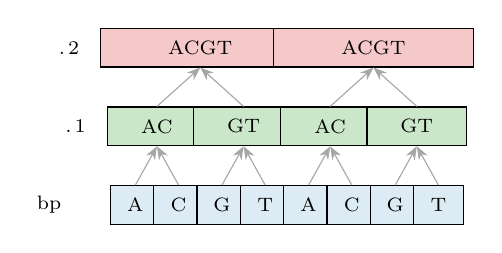
\begin{tikzpicture}[
    node distance=4pt and 2pt,
    bp/.style={draw, fill=accentBlue!15, minimum width=18pt, minimum height=14pt, font=\scriptsize},
    tok/.style={draw, fill=accentGreen!25, minimum width=36pt, minimum height=14pt, font=\scriptsize},
    big/.style={draw, fill=accentRed!25, minimum width=72pt, minimum height=14pt, font=\scriptsize},
    arr/.style={->, >=Stealth, thin, gray!70},
  ]
    % bp level
    \foreach \i/\ch in {0/A,1/C,2/G,3/T,4/A,5/C,6/G,7/T} {
      \node[bp] (b\i) at (\i*0.55, 0) {\ch};
    }
    \node[left=14pt of b0] {\scriptsize bp};

    % level 1
    \node[tok] (t0) at (0.275, 1.0) {AC};
    \node[tok] (t1) at (1.375, 1.0) {GT};
    \node[tok] (t2) at (2.475, 1.0) {AC};
    \node[tok] (t3) at (3.575, 1.0) {GT};
    \node[left=4pt of t0] {\scriptsize ур.\,1};
    \foreach \i/\j in {0/0,1/0,2/1,3/1,4/2,5/2,6/3,7/3}
      \draw[arr] (b\i.north) -- (t\j.south);

    % level 2
    \node[big] (u0) at (0.825, 2.0) {ACGT};
    \node[big] (u1) at (3.025, 2.0) {ACGT};
    \node[left=4pt of u0] {\scriptsize ур.\,2};
    \foreach \i/\j in {0/0,1/0,2/1,3/1}
      \draw[arr] (t\i.north) -- (u\j.south);
  \end{tikzpicture}
  \medskip
  \begin{itemize}
    \item На каждом уровне $\le 50\%$ позиций сливается.
    \item Глубина иерархии $K = \lceil \log_2 (L / T_{\text{target}}) \rceil$.
  \end{itemize}
\end{frame}

\begin{frame}{Дифференцируемый DP (dDP)}
  Задача: выбрать $\le k$ \emph{непересекающихся} пар, максимизирующих
  $\sum_{i \in S} s_i$, $|S| \le k$, $\forall i, j \in S: |i-j| \ge 2$.
  \medskip
  \textbf{Hard DP} (бэктрейс на дискретной маске):
  \[
    H[i, k] = \max\!\big(\,H[i-1, k],\; H[i-2, k-1] + s_{i-2}\,\big),
  \]
  \[
    H[0,0] = H[1,0] = 0,\quad \text{иначе } -\infty.
  \]

  \begin{itemize}
    \item DP запускается под \texttt{torch.no\_grad}.
    \item Градиент в $\theta$ течёт через \textbf{вспомогательную
          BCE-функцию} на сырых оценках $s_i$ против полученной маски.
    \item Оконный вариант \textbf{ddp\_windowed} для $L > 32k$ ---
          сегментация без потери асимптотики.
  \end{itemize}
\end{frame}

% --- 5. Architecture / training -------------------------------------------
\section{Архитектура и обучение}

\begin{frame}{Полная архитектура}
  \centering
  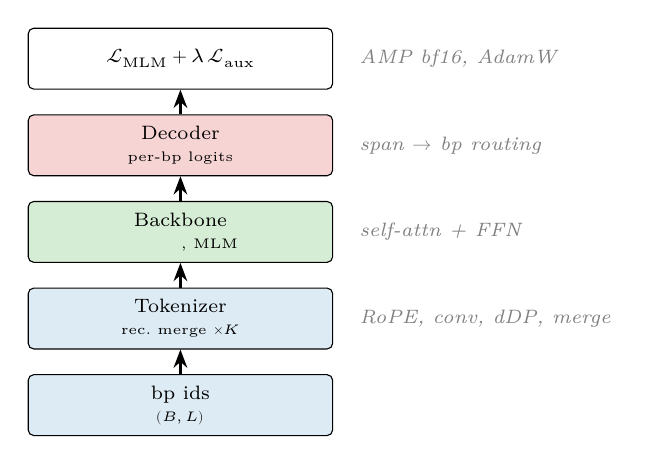
\begin{tikzpicture}[
    box/.style={draw, rounded corners=2pt, minimum width=110pt, minimum height=22pt, align=center, font=\scriptsize},
    arr/.style={->, >=Stealth, thick},
    note/.style={font=\scriptsize\itshape, gray},
  ]
    \node[box, fill=accentBlue!15] (in)  at (0,0)   {bp ids \\ \tiny $(B, L)$};
    \node[box, fill=accentBlue!15] (tok) at (0,1.1) {Tokenizer \\ \tiny rec.\ merge $\times K$};
    \node[box, fill=accentGreen!20] (bb) at (0,2.2) {Backbone \\ \tiny двунаправленный, MLM};
    \node[box, fill=accentRed!20] (dec) at (0,3.3) {Decoder \\ \tiny per-bp logits};
    \node[box] (loss) at (0,4.4) {$\mathcal{L}_{\text{MLM}} + \lambda\,\mathcal{L}_{\text{aux}}$};

    \draw[arr] (in)  -- (tok);
    \draw[arr] (tok) -- (bb);
    \draw[arr] (bb)  -- (dec);
    \draw[arr] (dec) -- (loss);

    \node[note, right=6pt of tok]  {RoPE, conv, dDP, merge};
    \node[note, right=6pt of bb]   {self-attn + FFN};
    \node[note, right=6pt of dec]  {span $\to$ bp routing};
    \node[note, right=6pt of loss] {AMP bf16, AdamW};
  \end{tikzpicture}
\end{frame}

\begin{frame}{Целевая функция}
  \textbf{MLM (Devlin et al.)}
  \[
    \mathcal{L}_{\text{MLM}}
    = -\frac{1}{|\mathcal{M}|} \sum_{i \in \mathcal{M}}
        \log p_\theta(x_i \mid x_{\setminus \mathcal{M}}),
  \]
  $\mathcal{M}$: 15\% позиций, из них 80\% $\to$ \texttt{[MASK]},
  10\% случайных, 10\% без изменений.

  \medskip
  \textbf{Вспомогательная BCE на оценках слияний}
  \[
    \mathcal{L}_{\text{aux}}
    = \sum_{\ell=1}^{K} \mathrm{BCE}\!\big(\sigma(s^{(\ell)}),\, m^{(\ell)}\big),
    \quad m^{(\ell)} = \mathrm{dDP}(s^{(\ell)}).
  \]

  \medskip
  \textbf{Полный лосс}
  \[
    \mathcal{L} = \mathcal{L}_{\text{MLM}} + \lambda\, \mathcal{L}_{\text{aux}},
    \qquad \lambda \in \{0,\, 0.5,\, 1.0\} \;\text{(абляция)}.
  \]
\end{frame}

\begin{frame}{Конфигурация обучения}
  \begin{itemize}
    \item \textbf{Оптимизатор}: AdamW (Loshchilov \& Hutter, 2019),
          $\beta = (0.9, 0.95)$, weight decay $0.1$ только для матриц.
    \item \textbf{LR}: warmup-linear $\to$ cosine decay (Loshchilov, 2017),
          $\text{min\_lr\_ratio} = 0.1$.
    \item \textbf{AMP}: bf16 (Micikevicius et al., 2018).
    \item \textbf{Параллелизм}: GPU-only, gradient accumulation, опционально
          PyTorch Lightning.
    \item \textbf{Гиперпараметры}: $d=256$, $L_{\text{layer}}=6$,
          $H=8$, $T=2048$, $T_{\text{target}}=512$, $\text{vocab}=9$.
    \item \textbf{Логирование}: MLflow (sqlite backend) + структурированные
          логи (loguru) в \texttt{outputs/runs/<run\_id>}.
  \end{itemize}
\end{frame}

% --- 6. Data / benchmarks --------------------------------------------------
\section{Данные и бенчмарки}

\begin{frame}{Корпус для предобучения --- T2T-CHM13}
  \begin{itemize}
    \item \textbf{T2T-CHM13 v2.0 (no Y)} --- первая полная сборка генома
          человека (Nurk et al., \emph{Science}, 2022).
    \item Размер: $\approx 2{,}9 \cdot 10^9$ bp непрерывной
          последовательности.
    \item Стриминговый \texttt{Dataset}: индекс $(file, offset, length)$
          строится один раз, окна читаются с диска по требованию ---
          память $O(\text{\# контигов})$ независимо от \texttt{num\_workers}.
    \item Загрузка: \texttt{httpx} стрим $\to$ gzip декодер $\to$ atomic
          \texttt{os.replace}; \texttt{tenacity} для ретраев.
  \end{itemize}
\end{frame}

\begin{frame}{Бенчмарки для оценки}
  \begin{tabular}{@{}lll@{}}
    \toprule
    Бенчмарк & Источник & Тип задач \\
    \midrule
    Genomic Benchmarks & Grešová et al., 2023 & 9 бинарных классификаций \\
    NT Downstream      & Dalla-Torre et al., 2024 & 18 задач (HF datasets) \\
    DART-Eval          & Patel et al., NeurIPS 2024 & 5 задач, регуляторная ДНК \\
    BEND               & Marin et al., ICLR 2024  & 7 биологических задач \\
    \bottomrule
  \end{tabular}
  \medskip
  \begin{itemize}
    \item Zero-shot оценка через MLM-правдоподобие
          (стиль DART-Eval Tier A).
    \item Каждый бенчмарк --- отдельный пакет с \texttt{tasks/}; одна
          задача = один файл, наследник \texttt{Task} ABC.
    \item Аутентификация: \texttt{SYNAPSE\_AUTH\_TOKEN} (DART-Eval),
          \texttt{HF\_TOKEN} (NT) --- через общий \texttt{.env.shared}.
  \end{itemize}
\end{frame}

% --- 7. Infrastructure -----------------------------------------------------
\section{Инфраструктура}

\begin{frame}[fragile]{Plug-and-play через Hydra}
\begin{lstlisting}[language=bash]
# train MLM с char baseline, MLflow tracker, sqlite backend
make train MODEL=char EXTRA="trainer.max_iters=50000"

# смена backbone и трекера без правок кода
make train MODEL=recursive trainer=lightning tracker=wandb

# eval с автоматическим выбором лучшего чекпойнта
make eval MODEL=recursive
\end{lstlisting}
  \begin{itemize}
    \item Каждый компонент --- yaml с \texttt{\_target\_:},
          \texttt{main.py} --- 88 LOC, никаких \texttt{isinstance}.
    \item Воспроизводимость: полный конфиг сохраняется в
          \texttt{<run\_dir>/config.yaml} и встраивается в каждый
          \texttt{checkpoint.pt}.
    \item Качество кода: mypy strict + ruff (Google docstrings) +
          pytest (109 тестов, $\ge 80\%$ покрытия) через \texttt{make check}.
  \end{itemize}
\end{frame}

\begin{frame}{Воспроизводимость и эксперименты}
  \begin{itemize}
    \item Один корень для артефактов: \texttt{outputs/\{runs, mlflow, benchmarks\}}.
    \item \texttt{run\_id} = \texttt{<дата>\_<время>\_<модель>} ---
          параллельные запуски разных моделей не конфликтуют.
    \item Long-running таргеты в tmux:
          \texttt{dna\_llm-train-<MODEL>}, \texttt{dna\_llm-eval-<MODEL>}.
    \item Загрузка данных: streaming + \texttt{tenacity} retry +
          атомарный rename, \texttt{FORCE=1} для перезагрузки.
    \item Все цитируемые работы $\to$ \texttt{references.bib} +
          inline-комментарии в коде (\texttt{\#~Author Year --
          (bibkey)}).
  \end{itemize}
\end{frame}

% --- 8. Status / next steps -----------------------------------------------
\section{Статус и план}

\begin{frame}{Текущий статус}
  \textbf{Готово}
  \begin{itemize}
    \item Архитектура адаптивного токенизатора (dDP, hierarchical merge,
          span-routed декодер).
    \item MLM-тренировка с поддержкой char / BPE / recursive backbone.
    \item Полный пайплайн данных и оценки, 4 бенчмарка как
          plug-and-play модули.
    \item Инфраструктура: тесты, типизация, CI-готовый \texttt{make check},
          Docker-like воспроизводимость через \texttt{uv}.
  \end{itemize}
  \medskip
  \textbf{В процессе}
  \begin{itemize}
    \item Первичные runs на CHM13 (char baseline уже обучается).
    \item Wiring DART-Eval Synapse-данных и зеро-шот оценки.
  \end{itemize}
\end{frame}

\begin{frame}{План до защиты}
  \begin{enumerate}
    \item Завершить претрейн на CHM13 для трёх моделей (char, BPE,
          recursive) с одинаковым бюджетом токенов.
    \item Прогнать Genomic Benchmarks и NT (zero-shot likelihood).
    \item Подключить DART-Eval Tier A (Tasks 1, 2, 5).
    \item Абляции: $\lambda \in \{0, 0.5, 1.0\}$,
          $T_{\text{target}} \in \{256, 512, 1024\}$, глубина иерархии.
    \item Провести анализ полученных слияний (биологическая
          интерпретируемость).
    \item Финальный текст диссертации, итоговые графики, защита.
  \end{enumerate}
\end{frame}

% --- Closing ---------------------------------------------------------------
\begin{frame}[standout]
  Спасибо за внимание! \\[0.4em]
  \large Вопросы?
\end{frame}

\end{document}
